\subsection{Convolutional Neural Network}
\label{subsec:cnn}
% \todo[inline]{Citations}

Convolutional neural networks are a type of deep learning architecture that is primarily used to classify images.
They are based on artificial neural networks and the mathematical convolution operation.
The efficiency in image classification of CNNs is largely responsible for the reputation of deep learning.
% https://pathmind.com/wiki/convolutional-network

The main problems when working with color images is that they are high-dimensional and therefore require a lot of processing power.
For this reason, convolutional neural networks use special layers to detect features and reduce the amount of data.
The three different layers used are convolution layers, pooling layers and fully-connected layers.
An example of a CNN sequence to classify handwritten digits is shown in figure \ref{fig:cnn}.
% https://pathmind.com/wiki/convolutional-network

\paragraph{Convolution Layer}
The convolution layer performs the convolution operations using so-called kernels or filters.
The goal of the convolution operation is to extract certain features --- such as edges --- from the image.
Different kernels are used to detect different features.
The first convolution layers are responsible for capturing low-level features, while following layers are responsible for capturing high-level features.
\clearpage
% https://towardsdatascience.com/a-comprehensive-guide-to-convolutional-neural-networks-the-eli5-way-3bd2b1164a53

\paragraph{Pooling Layer}
The pooling layers reduce the spatial size of the convolved features.
Pooling only looks at the portion of the image that is covered by the kernel.
Pooling is done by only looking at the portion of the image masked by the kernel.
Maximum pooling yields the maximum value and average pooling yields the average value of the masked portion.
By doing so, the required computational power is significantly decreases and the dominat features are extracted.
% https://towardsdatascience.com/a-comprehensive-guide-to-convolutional-neural-networks-the-eli5-way-3bd2b1164a53
\\

\paragraph{Fully-Connected Layer}
The fully-connected layers are responsible for learning the non-linear combinations of the high-level convolved features.
They flatten the result of the convolution process into a vector of values.
Each value corresponds to a probability that a certain feature belongs to a certain label.
% https://towardsdatascience.com/a-comprehensive-guide-to-convolutional-neural-networks-the-eli5-way-3bd2b1164a53

% https://towardsdatascience.com/a-comprehensive-guide-to-convolutional-neural-networks-the-eli5-way-3bd2b1164a53
\begin{figure}[t]
  \centering
  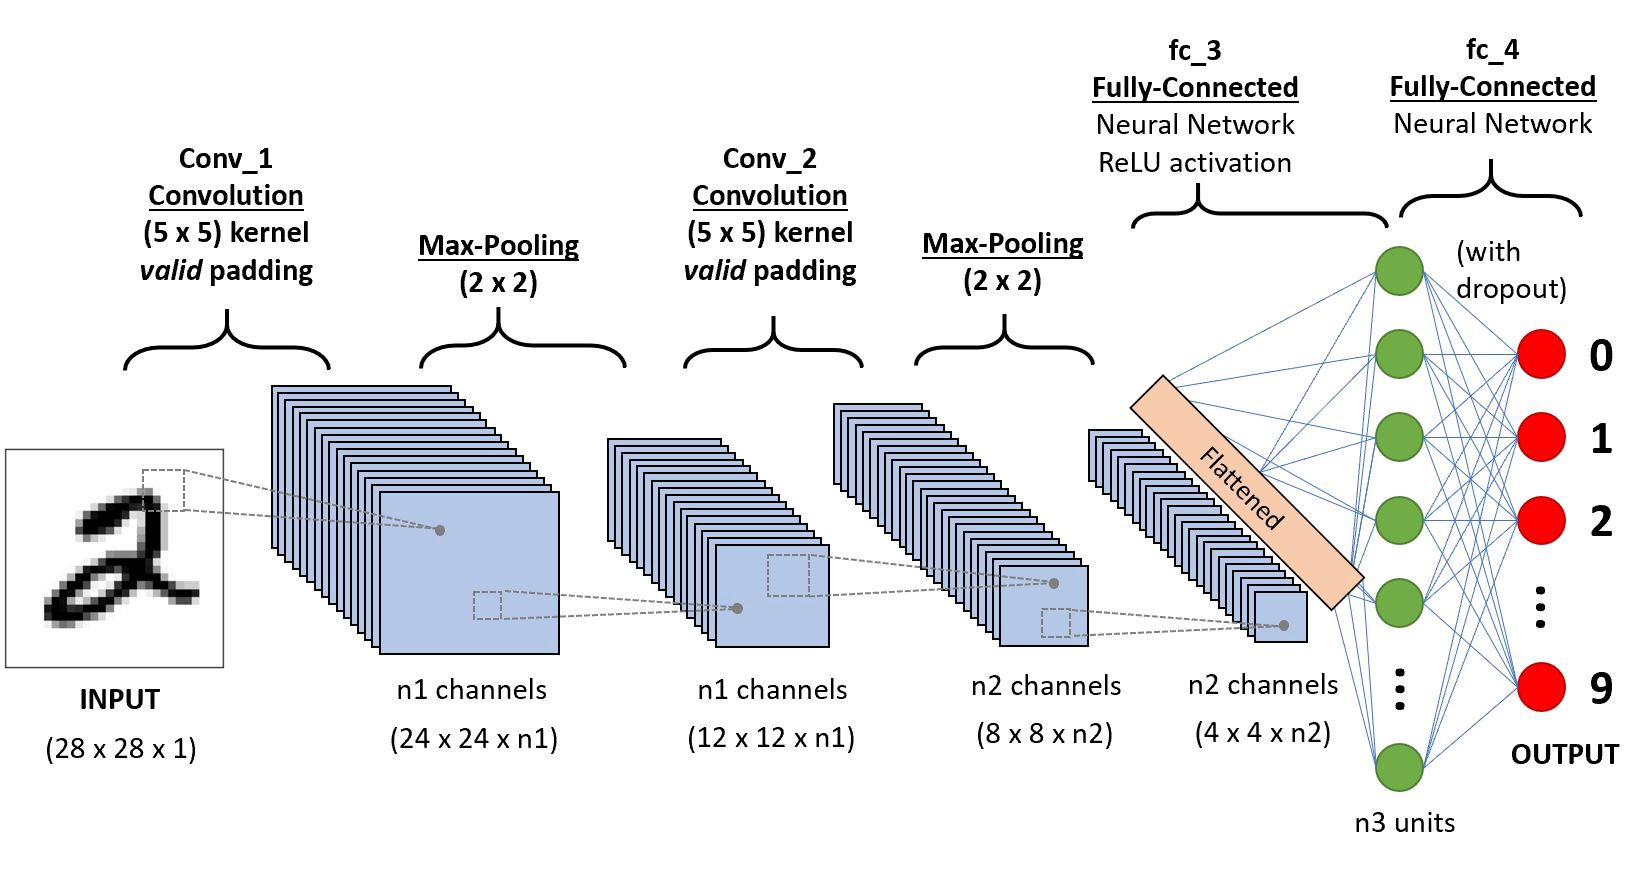
\includegraphics[width=\textwidth]{cnn}
  \caption{Example of a convolutional neural network}
  \label{fig:cnn}
\end{figure}
